\subsection{Db\-Image  Class Reference}
\label{class_dbimage}\index{DbImage@{Db\-Image}}
{\tt \#include $<$dbimage.h$>$}

Inheritance diagram for Db\-Image::\begin{figure}[H]
\begin{center}
\leavevmode
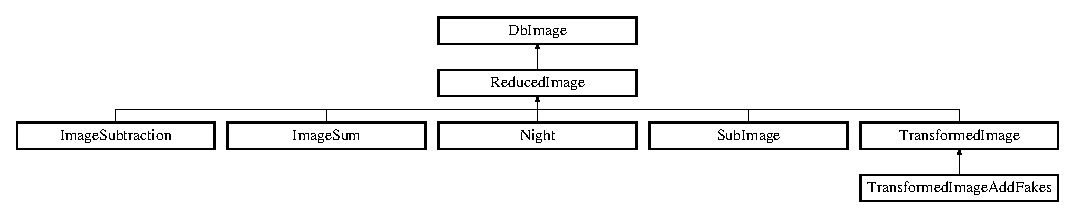
\includegraphics[height=2.47514cm]{class_dbimage}
\end{center}
\end{figure}
\subsubsection*{Public Methods}
\begin{CompactItemize}
\item 
\index{DbImage@{DbImage}!DbImage@{Db\-Image}}\index{DbImage@{DbImage}!DbImage@{Db\-Image}}
{\bf Db\-Image} (const string \&Image\-Name)\label{class_dbimage_a0}

\begin{CompactList}\small\item\em a constructor: its argument is a unique image identifier (eg r124280).\item\end{CompactList}\item 
\index{DbImage@{DbImage}!DbImage@{Db\-Image}}\index{DbImage@{DbImage}!DbImage@{Db\-Image}}
{\bf Db\-Image} (const char $\ast$Image\-Name)\label{class_dbimage_a1}

\begin{CompactList}\small\item\em a constructor: its argument is a unique image identifier (eg r124280).\item\end{CompactList}\item 
\index{DbImage@{DbImage}!DbImage@{Db\-Image}}\index{DbImage@{DbImage}!DbImage@{Db\-Image}}
{\bf Db\-Image} ()\label{class_dbimage_a2}

\item 
\index{IsValid@{IsValid}!DbImage@{Db\-Image}}\index{DbImage@{DbImage}!IsValid@{Is\-Valid}}
bool {\bf Is\-Valid} () const\label{class_dbimage_a3}

\begin{CompactList}\small\item\em for images obtained from the above constructor, checks that the image could be located.\item\end{CompactList}\item 
\index{Name@{Name}!DbImage@{Db\-Image}}\index{DbImage@{DbImage}!Name@{Name}}
string {\bf Name} () const\label{class_dbimage_a4}

\begin{CompactList}\small\item\em returns the image name.\item\end{CompactList}\item 
\index{Dir@{Dir}!DbImage@{Db\-Image}}\index{DbImage@{DbImage}!Dir@{Dir}}
string {\bf Dir} () const\label{class_dbimage_a5}

\item 
\index{DbImage@{DbImage}!DbImage@{Db\-Image}}\index{DbImage@{DbImage}!DbImage@{Db\-Image}}
{\bf Db\-Image} (const string \&Image\-Name, const Path $\ast$APath)\label{class_dbimage_a6}

\item 
\index{operator==@{operator==}!DbImage@{Db\-Image}}\index{DbImage@{DbImage}!operator==@{operator==}}
bool {\bf operator==} (const Db\-Image \&Right) const\label{class_dbimage_a7}

\begin{CompactList}\small\item\em to tell if we have twice the same image.\item\end{CompactList}\item 
string {\bf Fits\-Image\-Name} (const Db\-Image\-Kind Kind) const
\begin{CompactList}\small\item\em returns the {\bf Fits\-Image} {\rm (p.\,\pageref{class_fitsimage})} file name (a file name for the file system).\item\end{CompactList}\item 
\index{ElixirName@{ElixirName}!DbImage@{Db\-Image}}\index{DbImage@{DbImage}!ElixirName@{Elixir\-Name}}
string {\bf Elixir\-Name} () const\label{class_dbimage_a9}

\begin{CompactList}\small\item\em out of elixir name.\item\end{CompactList}\item 
string {\bf Image\-Back\-Name} (const Db\-Image\-Kind Kind) const
\begin{CompactList}\small\item\em same for the {\bf Image\-Back} {\rm (p.\,\pageref{class_imageback})} (background value and rms interpolated map).\item\end{CompactList}\item 
\index{FitsFlatName@{FitsFlatName}!DbImage@{Db\-Image}}\index{DbImage@{DbImage}!FitsFlatName@{Fits\-Flat\-Name}}
string {\bf Fits\-Flat\-Name} () const\label{class_dbimage_a11}

\begin{CompactList}\small\item\em the name of the fits file containig the flatfield used for flatfielding.\item\end{CompactList}\item 
\index{FitsBiasName@{FitsBiasName}!DbImage@{Db\-Image}}\index{DbImage@{DbImage}!FitsBiasName@{Fits\-Bias\-Name}}
string {\bf Fits\-Bias\-Name} () const\label{class_dbimage_a12}

\begin{CompactList}\small\item\em same for bias.\item\end{CompactList}\item 
\index{FitsDarkName@{FitsDarkName}!DbImage@{Db\-Image}}\index{DbImage@{DbImage}!FitsDarkName@{Fits\-Dark\-Name}}
string {\bf Fits\-Dark\-Name} () const\label{class_dbimage_a13}

\begin{CompactList}\small\item\em same for dark.\item\end{CompactList}\item 
\index{FitsWeightName@{FitsWeightName}!DbImage@{Db\-Image}}\index{DbImage@{DbImage}!FitsWeightName@{Fits\-Weight\-Name}}
string {\bf Fits\-Weight\-Name} () const\label{class_dbimage_a14}

\begin{CompactList}\small\item\em name of the weight imag.\item\end{CompactList}\item 
\index{FitsDeadName@{FitsDeadName}!DbImage@{Db\-Image}}\index{DbImage@{DbImage}!FitsDeadName@{Fits\-Dead\-Name}}
string {\bf Fits\-Dead\-Name} () const\label{class_dbimage_a15}

\begin{CompactList}\small\item\em same for dead pixel map.\item\end{CompactList}\item 
\index{FitsBadName@{FitsBadName}!DbImage@{Db\-Image}}\index{DbImage@{DbImage}!FitsBadName@{Fits\-Bad\-Name}}
string {\bf Fits\-Bad\-Name} () const\label{class_dbimage_a16}

\begin{CompactList}\small\item\em same for bad pixel map (built from weight map).\item\end{CompactList}\item 
\index{FitsCosmicName@{FitsCosmicName}!DbImage@{Db\-Image}}\index{DbImage@{DbImage}!FitsCosmicName@{Fits\-Cosmic\-Name}}
string {\bf Fits\-Cosmic\-Name} () const\label{class_dbimage_a17}

\begin{CompactList}\small\item\em same for cosmic pixel map.\item\end{CompactList}\item 
\index{FitsSatelliteName@{FitsSatelliteName}!DbImage@{Db\-Image}}\index{DbImage@{DbImage}!FitsSatelliteName@{Fits\-Satellite\-Name}}
string {\bf Fits\-Satellite\-Name} () const\label{class_dbimage_a18}

\begin{CompactList}\small\item\em same for satellite pixel map.\item\end{CompactList}\item 
\index{FitsFringeName@{FitsFringeName}!DbImage@{Db\-Image}}\index{DbImage@{DbImage}!FitsFringeName@{Fits\-Fringe\-Name}}
string {\bf Fits\-Fringe\-Name} () const\label{class_dbimage_a19}

\begin{CompactList}\small\item\em same for fringe pattern map map.\item\end{CompactList}\item 
\index{FitsBackName@{FitsBackName}!DbImage@{Db\-Image}}\index{DbImage@{DbImage}!FitsBackName@{Fits\-Back\-Name}}
string {\bf Fits\-Back\-Name} () const\label{class_dbimage_a20}

\begin{CompactList}\small\item\em background image.\item\end{CompactList}\item 
\index{FitsMiniBackName@{FitsMiniBackName}!DbImage@{Db\-Image}}\index{DbImage@{DbImage}!FitsMiniBackName@{Fits\-Mini\-Back\-Name}}
string {\bf Fits\-Mini\-Back\-Name} () const\label{class_dbimage_a21}

\begin{CompactList}\small\item\em min background image.\item\end{CompactList}\item 
\index{FitsSaturName@{FitsSaturName}!DbImage@{Db\-Image}}\index{DbImage@{DbImage}!FitsSaturName@{Fits\-Satur\-Name}}
string {\bf Fits\-Satur\-Name} () const\label{class_dbimage_a22}

\begin{CompactList}\small\item\em same for saturated stars pixels map.\item\end{CompactList}\item 
\index{ImageMatchUsnoName@{ImageMatchUsnoName}!DbImage@{Db\-Image}}\index{DbImage@{DbImage}!ImageMatchUsnoName@{Image\-Match\-Usno\-Name}}
string {\bf Image\-Match\-Usno\-Name} () const\label{class_dbimage_a23}

\begin{CompactList}\small\item\em return the results of the usno match.\item\end{CompactList}\item 
string {\bf Image\-Catalog\-Name} (const Db\-Image\-Catalog\-Kind Kind=SExtractor) const
\begin{CompactList}\small\item\em returns the list of stars detected and measured on the {\bf Image} {\rm (p.\,\pageref{class_image})} (a file name for the file system).\item\end{CompactList}\item 
\index{ImagePsfName@{ImagePsfName}!DbImage@{Db\-Image}}\index{DbImage@{DbImage}!ImagePsfName@{Image\-Psf\-Name}}
string {\bf Image\-Psf\-Name} (const Db\-Image\-Psf\-Kind Kind=Daophot\-Psf) const\label{class_dbimage_a25}

\begin{CompactList}\small\item\em returns the name where the psf parameters and look-up table for residuals is stored.\item\end{CompactList}\item 
\index{EverythingElseFileName@{EverythingElseFileName}!DbImage@{Db\-Image}}\index{DbImage@{DbImage}!EverythingElseFileName@{Everything\-Else\-File\-Name}}
string {\bf Everything\-Else\-File\-Name} () const\label{class_dbimage_a26}

\item 
\index{Create@{Create}!DbImage@{Db\-Image}}\index{DbImage@{DbImage}!Create@{Create}}
bool {\bf Create} (const string \&Path)\label{class_dbimage_a27}

\begin{CompactList}\small\item\em To create the directories where the fits images, catalogues will be put: ex: $\sim$/Fake\-Db/test: Db\-Image dbim(\char`\"{}test\char`\"{}); dbim.Create(\char`\"{}$\sim$/Fake\-Db/\char`\"{});.\item\end{CompactList}\item 
\index{GetFileName@{GetFileName}!DbImage@{Db\-Image}}\index{DbImage@{DbImage}!GetFileName@{Get\-File\-Name}}
string {\bf Get\-File\-Name} (const char $\ast$Which\-File) const\label{class_dbimage_a28}

\item 
\index{dump@{dump}!DbImage@{Db\-Image}}\index{DbImage@{DbImage}!dump@{dump}}
void {\bf dump} (ostream \&stream=cout) const\label{class_dbimage_a29}

\item 
\index{~DbImage@{$\sim$DbImage}!DbImage@{Db\-Image}}\index{DbImage@{DbImage}!~DbImage@{$\sim$Db\-Image}}
{\bf $\sim$Db\-Image} ()\label{class_dbimage_a30}

\item 
\index{init_from_name@{init\_\-from\_\-name}!DbImage@{Db\-Image}}\index{DbImage@{DbImage}!init_from_name@{init\_\-from\_\-name}}
void {\bf init\_\-from\_\-name} ()\label{class_dbimage_a31}

\item 
\index{writeEverythingElse@{writeEverythingElse}!DbImage@{Db\-Image}}\index{DbImage@{DbImage}!writeEverythingElse@{write\-Everything\-Else}}
bool {\bf write\-Everything\-Else} ()\label{class_dbimage_a32}

\end{CompactItemize}
\subsubsection*{Protected Attributes}
\begin{CompactItemize}
\item 
\index{saveEverythingElse@{saveEverythingElse}!DbImage@{Db\-Image}}\index{DbImage@{DbImage}!saveEverythingElse@{save\-Everything\-Else}}
bool {\bf save\-Everything\-Else}\label{class_dbimage_n0}

\end{CompactItemize}
\subsubsection*{Friends}
\begin{CompactItemize}
\item 
class {\bf Db\-Image\-List}
\item 
class {\bf operator$<$$<$}
\end{CompactItemize}


\subsubsection{Detailed Description}
A Db\-Image refers to one image as the telescope provides it (more precisely, one CCD), together with associated data used for the reduction (flat and bias frames) or produced  during the reduction (lists of stars). 



\subsubsection{Member Function Documentation}
\index{DbImage@{Db\-Image}!FitsImageName@{FitsImageName}}
\index{FitsImageName@{FitsImageName}!DbImage@{Db\-Image}}
\paragraph{\setlength{\rightskip}{0pt plus 5cm}string Db\-Image::Fits\-Image\-Name (const Db\-Image\-Kind {\em Kind}) const}\hfill\label{class_dbimage_a8}


returns the {\bf Fits\-Image} {\rm (p.\,\pageref{class_fitsimage})} file name (a file name for the file system).

The Kind argument can be Raw or Flat\-Fielded. Nothing ensures that the file exists. One may use the File\-Exists routine  to check. \index{DbImage@{Db\-Image}!ImageBackName@{ImageBackName}}
\index{ImageBackName@{ImageBackName}!DbImage@{Db\-Image}}
\paragraph{\setlength{\rightskip}{0pt plus 5cm}string Db\-Image::Image\-Back\-Name (const Db\-Image\-Kind {\em Kind}) const}\hfill\label{class_dbimage_a10}


same for the {\bf Image\-Back} {\rm (p.\,\pageref{class_imageback})} (background value and rms interpolated map).

Same remark as above concerning the existence. \index{DbImage@{Db\-Image}!ImageCatalogName@{ImageCatalogName}}
\index{ImageCatalogName@{ImageCatalogName}!DbImage@{Db\-Image}}
\paragraph{\setlength{\rightskip}{0pt plus 5cm}string Db\-Image::Image\-Catalog\-Name (const Db\-Image\-Catalog\-Kind {\em Kind} = SExtractor) const}\hfill\label{class_dbimage_a24}


returns the list of stars detected and measured on the {\bf Image} {\rm (p.\,\pageref{class_image})} (a file name for the file system).

The Kind argument can be SExtractor or Fitted\_\-for\_\-seeing.  See Fits\-Image\-Name for caution instructions 

The documentation for this class was generated from the following file:\begin{CompactItemize}
\item 
{\bf dbimage.h}\end{CompactItemize}
